\documentclass[a4paper,12pt]{report}
 
\usepackage[utf8]{inputenc}
\usepackage[T1]{fontenc}
\usepackage[francais]{babel}
\usepackage{graphicx}
\usepackage{geometry}
\usepackage{lipsum}

\begin{document}

\begin{titlepage}
\begin{center}
{\Huge Projet autonome en Programmation C}\\[4ex] 
{\Huge \textbf{\textsc{EPIC} Giratoire Simulator}}\\[4ex] 
\today\\[8ex]
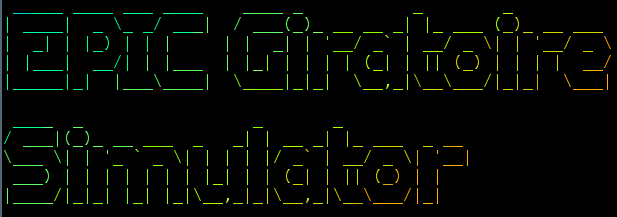
\includegraphics[scale=0.6]{logo2.png}\\[50ex]
\end{center}

\begin{tabular}{p{5cm} p{7cm}}
\vspace{0pt}
\textsc{BOUNIOL} Pierre\\\textsc{LE} Gregory
&
\vspace{0pt}
\hfill
\includegraphics[scale=0.2]{Logo-ESIEA.jpg}
\end{tabular}

\end{titlepage}

\renewcommand{\contentsname}{Sommaire}

\pagenumbering{gobble}
\tableofcontents
\newpage

\pagenumbering{arabic}
\newpage
\addcontentsline{toc}{part}{Introduction}
\chapter*{Introduction}
\paragraph{}
Dans le cadre du module \textsc{LAB3040 - Projet autonome en programmation C}, nous avons écrit un programme en langage C simulant le fonctionnement d'un carrefour giratoire. Ce programme devait proposer trois modes différents pour simuler trois densité de circulation : fluide, chargée et dangereuse.
\paragraph{}


\newpage
\addcontentsline{toc}{part}{Réalisation}
\chapter*{Réalisation}
\lipsum{1}

\newpage
\addcontentsline{toc}{part}{Difficultées rencontrées}
\chapter*{Difficultées rencontrées}
\lipsum{1}

\newpage
\addcontentsline{toc}{part}{Conclusion}
\chapter*{Conclusion}
\lipsum{1}

\end{document}